\documentclass{article}

% The preceding line is only needed to identify funding in the first footnote. If that is unneeded, please comment it out.
\usepackage{minted}
\usepackage{cite}
\usepackage{amsmath,amssymb,amsfonts}
\usepackage{algorithmic}
\usepackage{graphicx}
\usepackage{float}
\usepackage{textcomp}
\usepackage{xcolor}
\usepackage{outlines}
\usepackage{enumitem}
\setenumerate[1]{label=\arabic*.}
\setenumerate[2]{label=\alph*.}

\newcommand{\ket}[1]{{\lvert #1 \rangle}}
\newcommand{\bra}[1]{{\langle #1 \rvert}}
\newcommand{\braket}[2]{{\langle #1 \rvert #2 \rangle}}
\newcommand{\tr}{{\textrm{Tr}}}
\newcommand{\I}{{\mathbb{I}}}

\def\BibTeX{{\rm B\kern-.05em{\sc i\kern-.025em b}\kern-.08em
    T\kern-.1667em\lower.7ex\hbox{E}\kern-.125emX}}
\begin{document}
\begin{titlepage}
    \begin{center}
        \vspace{4cm}
        \large
        \textbf{
            Getting started coding quantum computers with QASM and Qiskit \\
            Initial research report \\
            Dylan Miracle \\
            ICS 698-02 \\
            Spring 2021 \\
            Mar 23, 2021 \\
            Dr. Jigang Liu
        }
    \end{center}
\end{titlepage}
\title{Getting started coding quantum computers with QASM and Qiskit}

\author{Dylan Miracle\\
\textit{Department of Computer Science} \\
\textit{Metropolitan State University}\\
St. Paul, Minnesota, USA \\
dylan.miracle@my.metrostate.edu
}

\maketitle

\tableofcontents
\pagebreak

\section{Introduction}

In the early days of digital computing a programmer needed a deep understanding of electrical engineering to program computers. The programming was low level involving digital logic gates and binary code. Abstractions were slowly built in to allow programmers to manipulate abstract data types so that now you can program a computer in a human readable language that uses high level concepts such as object inheritance and lambda calculus. Quantum computing is in its early phase and will likely progress to human human readable abstractions quickly. Developers who want to learn to program quantum computers will be served well to learn a programming framework to experiment with as opposed to taking a PhD in physics before learning the basics of quantum computing. It is not necessary to understand how a computer stores a string to build a web page, we should expect the same kinds of abstractions from quantum computing in the coming decade.

Frameworks such as qiskit and others already give a programmer access to many tools for interpreting and experimenting with quantum computers. This work aims to show an interested developer how to get started programming and interpreting quantum results. After reading this paper, for example, a developer would be able to create a webpage to display quantum results because they could understand how the result data is returned. Without needing to know the ins-and-outs of quantum computing they would be able to manipulate result data with a classical computer. This is a valuable tool because quantum computers will always be used with classical computers.

Quantum computing has a rich theoretical background but practical quantum computers have only recently become available to researchers and business users. These computers are still rare and operated by a small number of hardware vendors. The dominant paradigm for programing quantum computers is the gate model of quantum computing that defines a sequence of operations on a set of qubits. In this paper we introduce a fundamental quantum circuit and demonstrate its implementation using an intermediate representation, QASM, and a higher level quantum computing framework Qiskit. 

In this paper we will explore how quantum computing will fit into a standard computing workflow. 

This work gives an overview, from mathematical development of a simple quantum circuit to implementation with a high level quantum framework. Readers will get a taste of the complete quantum pipeline. This is valuable because much work focuses on one area of the ecosystem instead of walking those new to quantum mechanics through the complete process of how to implement some quantum code. For example, there are many papers detailing the use of a particular language, or that go into depth on specific quantum algorithms. Even though we focus on a specific framework the model of understanding quantum development proposed by this paper will be useful to anyone who wants to delve further into quantum computing. 

\section{Background}

A basic discussion of quantum computing will involve developing two fundamental concepts in quantum computing, namely superposition and entanglement.
Specifically we will use the example of the Bell states. These are the most basic states that exhibit the main features of quantum computing, namely superposition and entanglement of qubits. The development of this basic quantum circuit will start by exploring qubits and some basic quantum operations.

\subsection{Qubits}

Qubits are represented as two element column vectors. The elements are complex numbers. Since we measure qubits to be either 0 or 1 we will talk about them as being in the computational basis. This is not the only basis we can measure qubits. A single qubit can be visualized as a vector inside a unit sphere. This sphere is known as the Bloch sphere. 

\begin{figure}[H]
    \centering
    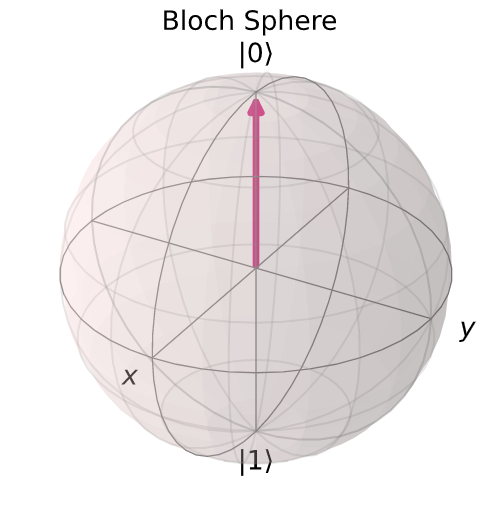
\includegraphics[width=0.25\textwidth]{bloch0.png}
    \caption{Bloch vector for qubit $\ket{0}$.}
\end{figure}

\begin{figure}[H]
    \centering
    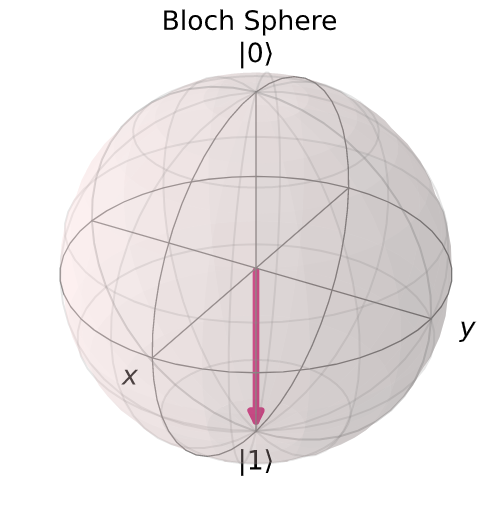
\includegraphics[width=0.25\textwidth]{bloch1.png}
    \caption{Bloch vector for qubit $\ket{1}$.}
\end{figure}

\begin{figure}[H]
    \centering
    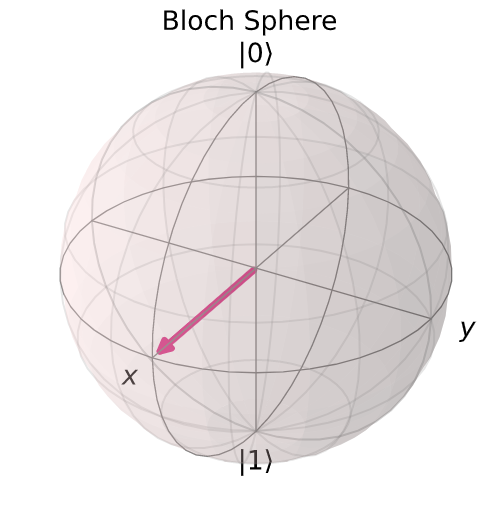
\includegraphics[width=0.25\textwidth]{superpos.png}
    \caption{Bloch vector for qubit $(\ket{0}+\ket{1})/\sqrt{2}$.}
\end{figure}

$$
\ket{0} = 
\begin{bmatrix}
1 \\
0
\end{bmatrix}
$$
$$
\ket{1} =
\begin{bmatrix}
0 \\
1
\end{bmatrix}
$$
$$
\frac{1}{\sqrt{2}}(\ket{0}+\ket{1}) = 
\begin{bmatrix}
    \frac{1}{\sqrt{2}}\\
    \frac{1}{\sqrt{2}}
\end{bmatrix}
$$
$$
H = \frac{1}{\sqrt{2}}
\begin{bmatrix}
    1 & 1 \\
    1 & -1
\end{bmatrix}
$$
% $$
% \texrm{CNOT} =
% \begin{bmatrix}
%     1 & 0 & 0 & 0 \\
%     1 & -1 \\

% \end{bmatrix}
% $$
\subsection{Bell state}

We achieve a bell state by using a CNOT gate to combine a $\ket{0}$ with a superposition like 
$\frac{1}{\sqrt{2}}(\ket{0}+\ket{1})$. This creates what is known as an entangled state. This combination results in a state represented as 

$$
\frac{\ket{00}+\ket{11}}{\sqrt{2}}
$$

With the property that any individual measurement of on of the qubits is random, but the measurement of the second qubit is entangled with the measurement of the first. So a measurement of 1 for qubit 0, means we will get a 1 for qubit 1 as well. In the next section we will simulate such a state and visualize it with a histogram.




\section{Preliminary findings}

\subsection{Quantum and classical workflows}

The central finding of this paper is that quantum computing will employ workflows from classical digital computers that software developers are used to using to implement new types of computation that will me new to most software developers. We show that the preparation of a quantum circuit is created with a domain specific language, then loaded into a python program that will look familiar to python developers. The quantum workload will be sent to a quantum backend where the quantum computation will be done, then the results will be collected into a data structure that can be analyzed and displayed using standard methods. We demonstrate a simple quantum program and decompose its workflow into the classical and quantum parts so that we can understand how developers will used quantum computing in the near future.

\subsection{Program bell state in QASM}

QASM is the basic assembly level intermediate representation for quantum code. It allows us to create two types of registries: quantum registries and classical registries. The quantum registries hold the information in qubits while the classical registries hold information in bits. Higher level languages use python libraries to represent the different parts of the quantum program.

Pure quantum computing involves superposition and entanglement. We will use a hybrid approach, preparing our problem on a classical computer, then submitting a job to a quantum computer, finally gathering and displaying our results using a classical computer. 

In this program we will implement the Bell state by preparing two quantum registers and two classical registers. The quantum registers will then be put into a Bell state by sending one qubit through a Hadamard gate to create a superposition, then both qubits through a CNOT gate to entangle them. Finally a measurement will be performed on each qubit independently. 
\begin{samepage}
\begin{figure}[H]
\begin{minted}{c}
OPENQASM 2.0;
include "qelib1.inc";

qreg q[2];
creg c[2];
h q[0];
cx q[0],q[1];
  
measure q[0] -> c[0];
measure q[1] -> c[1];
\end{minted}
\caption{bell.qasm}
\end{figure}
\end{samepage}

Once we have defined the circuit using the intermediate representation of QASM, we can import the circuit into a higher level language that will be used to submit the circuit to a simulator or to quantum hardware. In the following example we will use Qiskit to load our circuit and submit it to the builtin simulator.

\subsection{Load circuit into Qiskit and submit job}

The Qiskit program that follows will expand our workflow. We use standard methods of python programming familiar to anyone used to using the language to load our libraries, import the circuit, then submit the circuit to the simulator backend. The only change we would need to make to submit this program to actual quantum hardware is the change the backend to point at a quantum processor.

\begin{samepage}
\begin{figure}[H]
\begin{minted}{python}
import qiskit
from qiskit.visualization import plot_histogram

qc = qiskit.QuantumCircuit.from_qasm_file("bell.qasm")
qc.h(0)

backend = qiskit.Aer.get_backend('qasm_simulator')
result = qiskit.execute([qc], backend, shots=100)
count = result.result().get_counts()
plot_histogram(count)
\end{minted}
\caption{bell-qiskit.py}
\end{figure}
\end{samepage}

\subsection{Summary of findings}
By running our simulation 100 times we can gather statistics on the results of the measurements. Here is a histogram of measurements from the simulation shown

\begin{figure}[H]
    \centering
    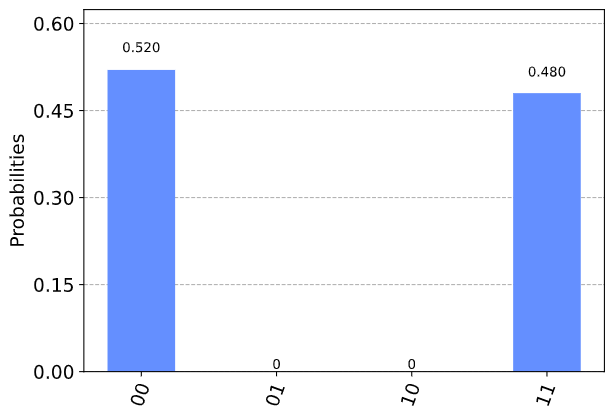
\includegraphics[width=0.75\textwidth]{histogram.png}
    \caption{Simulations of measurements of Bell state.}
\end{figure}

While QASM and Qiskit are specific to IBM, the model they use of intermediate representation and higher level language is present with other vendors (see Rigetti) and a good way to understand and control a quantum computer. An intermediate language gives us a method to write out specific gates used in most quantum computing algorithms, while the higher level framework lets us use standard computing. 



\section{Charts or tables}
\subsection{Circuit diagram}
This diagram shows the standard circuit representation for gate model quantum computing. This is a simple circuit that creates a Bell state with two starting qubits, then shows the measurements of those qubits being written into classical bits.
\begin{figure}[H]
    \centering
    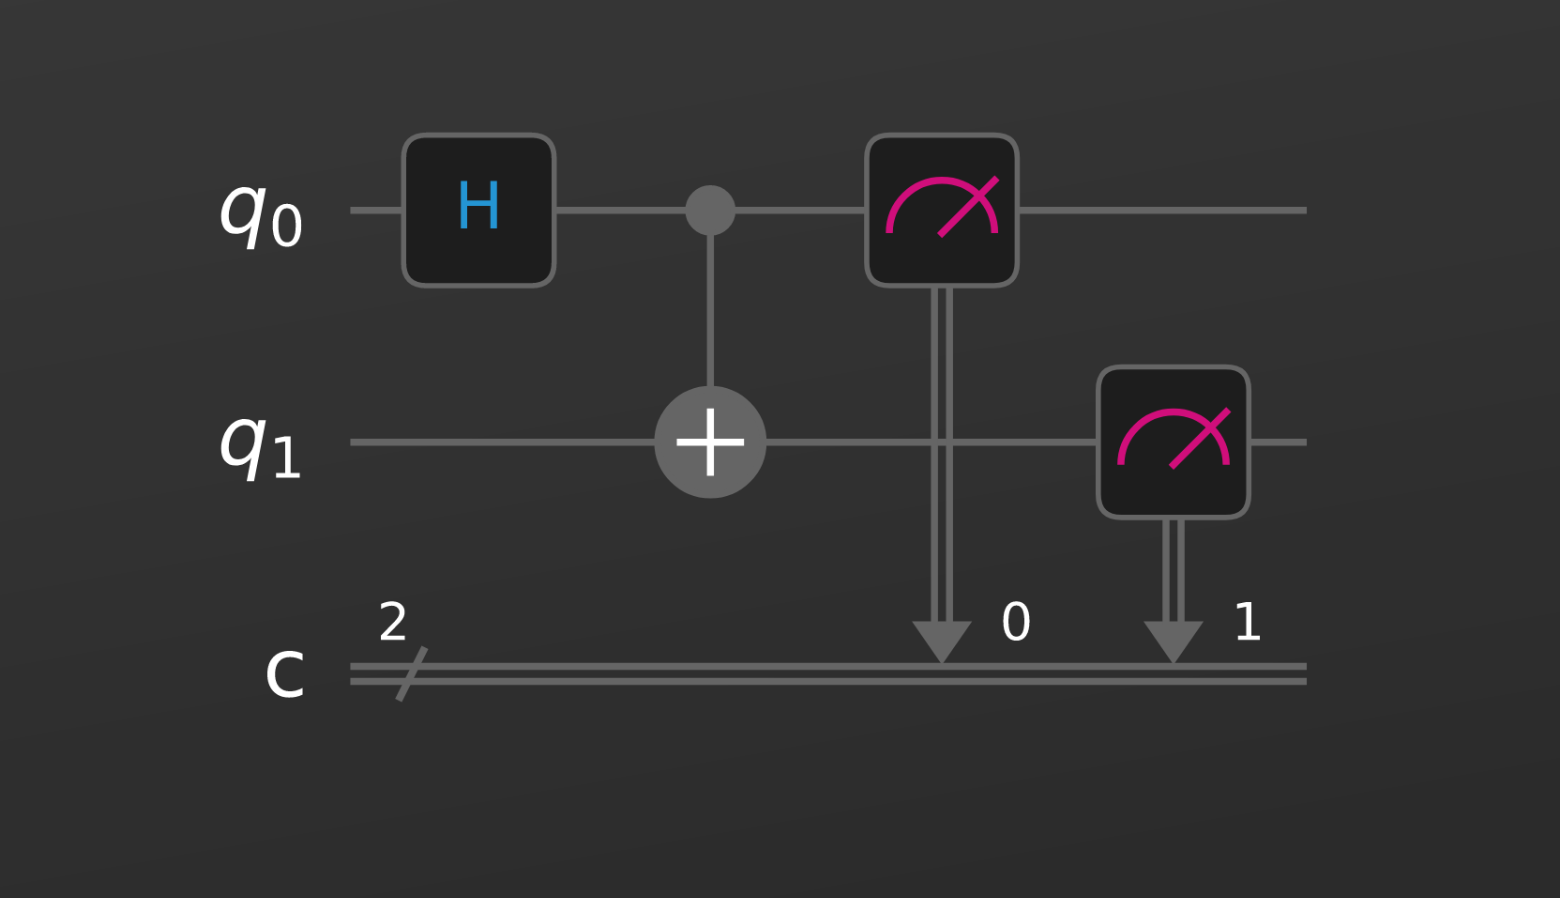
\includegraphics[width=0.75\textwidth]{circuit.png}
    \caption{A quantum circuit that will create a Bell state with two qubits.}
\end{figure}

\subsection{Quantum development flowchart}
Developing quantum algorithms is found to follow a flow from the quantum mechanics, to a quantum circuit, to intermediate representations, to higher level frameworks. This flow illustrates the findings of this paper and will serve as an outline for our exploration of quantum computing. 
\begin{figure}[H]
    \centering
    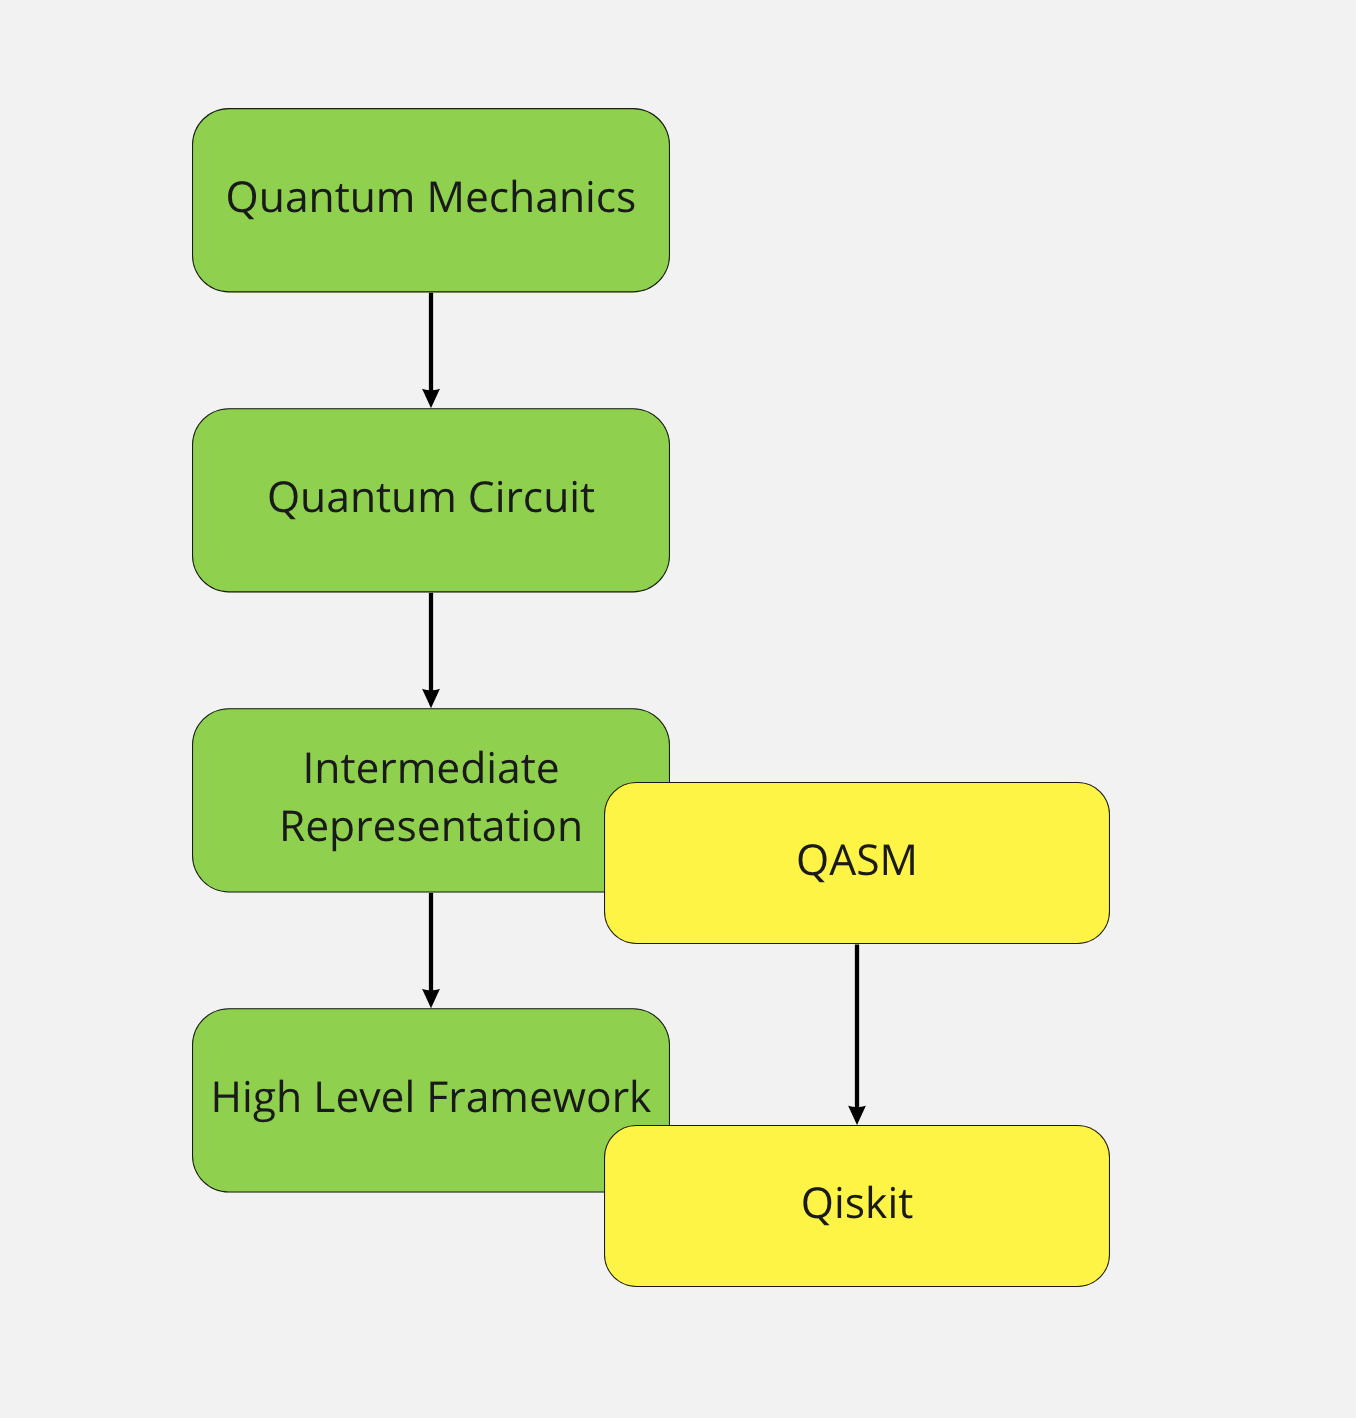
\includegraphics[width=0.75\textwidth]{flowchart.png}
    \caption{The quantum development flow.}
\end{figure}



\subsection{Quantum workflow flowchart}
Developing quantum algorithms is found to follow a flow from the quantum mechanics, to a quantum circuit, to intermediate representations, to higher level frameworks. This flow illustrates the findings of this paper and will serve as an outline for our exploration of quantum computing. 
\begin{figure}[H]
    \centering
    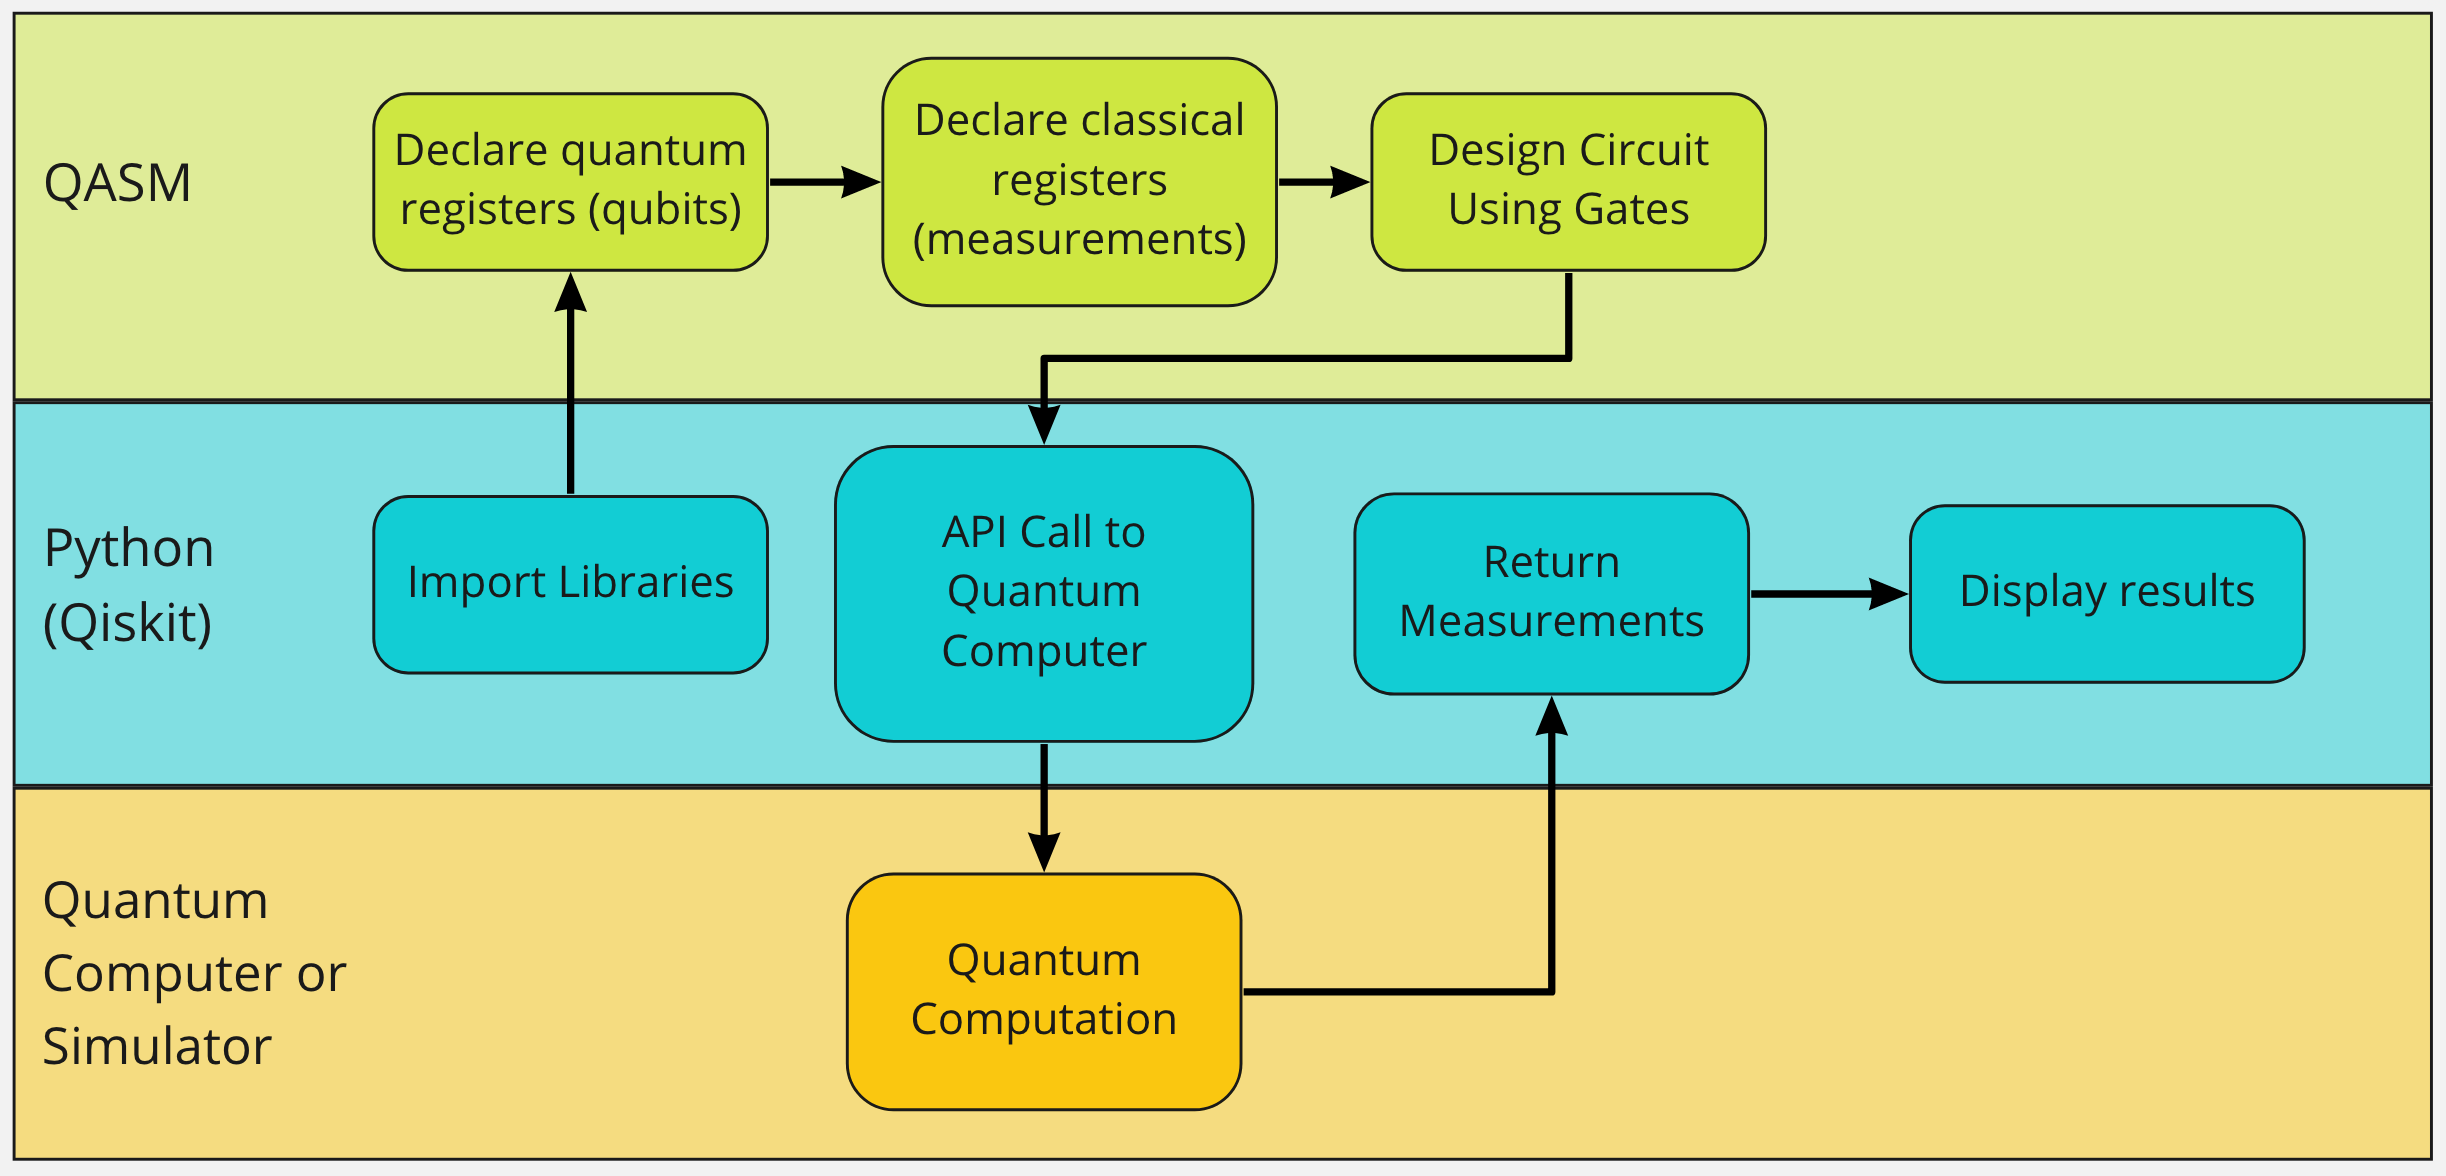
\includegraphics[width=1.0\textwidth]{qworkflow.png}
    \caption{The quantum computing workflow.}
\end{figure}

\section{Preliminary conclusion}

We should understand quantum computation as a workflow between the classical computer and the quantum computer. In this example we will create a simple quantum program and follow its execution using standard open source tooling available for programming IBM quantum computers. At the highest level we can understand that the classical computer is used to define the computation we will do, then an API is used to communicate the quantum job to the chosen backend, in our case a simulator, though a similar method will be used to submit the job to actual quantum hardware.


Developers can write code for quantum computers by learning frameworks in already existing languages. Several frameworks studied in the literature review have python frameworks. Python is often used because it is broadly adopted by the scientific community and creates a lower barrier to entry than some other languages might. For example Microsoft's Q\# language uses a combination of F\# and C\# that is less familiar to people not used to writing code in both of those languages. A good framework gives developers access to the tools needed to run quantum gates, but also standard computing tools that are helpful in interpreting results. The model used by qiskit to run jobs and return results means that programmers can predict what kind of data they will be dealing with before they fully understand the algorithms being used on the quantum side. As more software has a quantum components having well defined result data and job definitions means that software developers can create code for interpreting results and dealing with the output of quantum computers without becoming quantum computing experts.

Quantum computing will not stand on its own, but will always be employed in tandem with classical computing. This is as simple as using standard computers to create flow control or as advanced as using the fully featured APIs needed to connect to actual quantum hardware. As discussed the data returned by quantum algorithms will be interpreted and represented by classical computers. It is possible to currently develop software that will use quantum results in the future because well designed frameworks like qiskit have a standard workflow and results data structure.

Much work has been done to develop quantum computing frameworks. These frameworks are racing to increase functionality and capabilities for advanced users. This paper should give an overview of some of the fundamentals of quantum computing for an advanced undergraduate or software developer without a background in quantum mechanics. The audience for most quantum computing work is physics PhDs making it inaccessible to a typical software developer. This has a chilling effect on a bourgeoning industry. When we think about the great contributions to our modern information age we often end up thinking about hackers in a garage just as much as engineers in a clean room.

\section{Next Steps}

The next part of this study could be to extend our workflow understanding to encompass what tools are available to build hybrid workflows for the different kinds of quantum applications that will be available in the short term. The quantum computers that are available now are known as noisy intermediate scale quantum (NISQ) computers. These can only run a certain subset of quantum algorithms. Next steps would be to create workflows for NISQ computers.

\section{References}
\begin{thebibliography}{00}
    \makeatletter
    \makeatother
    \bibitem{b1} Michael S. Saraivanov, Quantum Circuit Synthesis using Group Decomposition and Hilbert Spaces, MS, Portland State University, 2013.
    \bibitem{b2} M. A. Nielsen and I. L. Chuang, Quantum Computation and Quantum Information, 10th Anniversary ed., Cambridge, 2016, pp. 171--215.
    \bibitem{b3} R. LaRose, ``Overview and Comparison of Gate Level Quantum Software'', Quantum Journal, 3/25/2019
    \bibitem{b4} F. Leymann, J. Barzen, ``Hybrid Quantum Applications Need Two Orchestrations in Superposition: A Software Architecture Perspective'', arXiv:quant-ph/2103.04320, 2021
    \bibitem{b5} Andrew W. Cross and Lev S. Bishop and John A. Smolin and Jay M. Gambetta, ``Open Quantum Assembly Language,'' arXiv:quant-ph/1707.03429, 2017.      
    \bibitem{b6} A. Asfaw, L. Bello, Y. Ben-Haim, M. Bozzo-Rey, S. Bravyi, N. Bronn, L. Capelluto, A. C. Vazquez, J. Ceroni, R. Chen, A. Frisch, J. Gambetta, S. Garion, L. Gil, S. De La Puente Gonzalez, F. Harkins, T. Imamichi, H. Kang, A. H. Karamlou, R. Loredo, D. McKay, A. Mezzacapo, Z. Minev, R. Movassagh, G. Nannicni, P. Nation, A. Phan, M. Pistoia, A. Rattew, J. Schaefer, J. Shabani, J. Smolin, J. Stenger, K. Temme, M. Tod, S. Wood, and J. Wootton., Learn Quantum Computation Using Qiskit, 2020, {http://community.qiskit.org/textbook}, University of Waterloo, 2008.
\end{thebibliography}
\end{document}
